% Glossary
%
% checkpoint =
% overhead = 
% resource = ressource
% grid = grid
% backtrack = 
% board = bræt 
% cornerboard = hjørnebræt (ikke ved kodehenvisning) 
% middleboard = midterbræt (ikke ved kodehenvisning)
% bitmap = bitmap
% bound =
% 


\documentclass[pdf,draft,a4paper,10pt]{article}
\usepackage[utf8]{inputenc}
\usepackage[danish]{babel}
\usepackage{natbib}
\bibliographystyle{dk-plainnat}



\usepackage{url}
\usepackage[final]{graphicx}
\usepackage{verbatim}
\usepackage{amssymb,amsmath}
\usepackage{lscape}
\usepackage{multicol}
\usepackage[draft]{fixme}
\usepackage{tikz}
\usetikzlibrary{trees}
%\usepackage{pgflibrarytikztrees}

\usepackage{listings}
\usepackage{fancyvrb}

\usepackage{wrapfig}                           %Mulighed for at wrappe tekst om figurer
\usepackage{fancyhdr}                          %Flere muligheder med headere og footere
\usepackage{lastpage}                          %Mulighed for at referere til sidste sidetal
\usepackage[final]{hyperref}


\newcommand{\mig}{MiG}
\newcommand{\oc}{One-Click}
\newcommand{\nq}{N-dronning-problemet}


%\headheight 14.5pt                             %H<F8>jden af headeren
%\textwidth 5.87in                              %Tekstbredden

%\oddsidemargin 0.2in                           %Venstre margin er 1in + dette tal
                                               %Med en textwidth p<E5> 5.87in og en
                                               %oddsidemargin p<E5> 0.2 bliver marginerne
                                               %lige store p<E5> A4 som er 8,27in bredt
\font\chessfont=skak10
\def\chs#1{{\chessfont#1}}

\renewcommand{\thepage}{\roman{page}}

\title{Bachelorprojekt\\N-dronning problemet i \mig}
\author{Thomas Clement Mogensen \\ Frej Soya \\ Alex Esmann }
\usepackage{amsmath}

\begin{document}

\maketitle
\tableofcontents
\newpage

\renewcommand{\thepage}{\arabic{page}}
\pagestyle{fancy}                              %Benyt fancyhdr-pakken
\fancyhead[R]{\thepage\ af \pageref{LastPage}} %Skriv sidetallene som "x af y"
\fancyhead[L]{\nq\ i \mig}              %Headeren
\fancyfoot[C]{}                                %Fjern sidetallet som er standard
\setcounter{page}{1}

\abstract
\begin{verse}
	En del af indholdet af problemformulereringen fra synopsen flyttes til henholdsvis resumé, \ref{nqueenproblemet} og \ref{migogoneclick}. Selve synopsen inkluderes som bilag. Resuméet skal være ren gentagelse.
\end{verse}
\fixme{slet?}
Projektets formål er ikke at beregne en løsning til \nq\ for $n=26$, hvilket problemets beregningsmæssige omfang kombineret med tids- og ressourcebegrænsninger udelukker i praksis. Men kun at muliggøre og forhåbentlig igangsætte denne beregning.
Vi vil ikke tage stilling til den benyttede algoritmes korrekthed eller effektivitet, men kun til den bedst mulige strategi for parallelisering. Partitionering af problemdata skal foregå på en fornuftig måde, med tanke på hvordan det forventes beregningsressourcerne opfører sig, men en decideret statisk undersøgelse af midlertidige \mig-ressourcers opførsel eller levetid vil ikke blive foretaget\footnote{Med ressourcers opførsel tænkes på den tid man kan forvente en bruger vil lade sin \oc-klient køre}. Fordele og ulemper ved \mig\ eller \oc\ i forhold til andre grid-systemer falder også udenfor opgavens omfang.

Ved at at løse problemet for et lavere $n$ vil vi kunne estimere tiden og/eller antal CPU'er der skal bruges for at løse for $n=26$.

 Opgaven behandler følgende delproblemer:
\begin{itemize}
\item At finde en effektiv strategi til parallelisering af Takakens algoritme. Herunder overvejelser omkring den optimale størrelse på delproblemer.
\item Implementation af algoritmen i java på en sådan måde at den kan afvikles af \oc-klienter.
\item Strategi for indsamling, behandling og præsentation af delresultater.
\item Første opgave er naturligvis at få et bedre kendskab til \mig.
\end{itemize}


\subsection*{Konklusion}\label{konklusion}
\begin{verse}
	Kortfattet konklusion på løsningen og processen
\end{verse}

\section{\nq}\label{nqueenproblemet}

\nq\ består i at finde antallet af måder man kan placerer $n$ dronninger på et et kvadratisk $N \times N$ bræt, således at ingen dronning kan slå en anden. Bemærk at vi skal finde alle løsninger, $Q(n)$, og ikke bare finde en løsning - hvilket er et helt andet problem. Hidtil er der kun fundet løsninger for $n \in \{1,...,25\}$ som kan findes i OIES databasen vedligeholdt af \citep{sekvenser}. Derudover beskriver \cite{etsi} en manuelt\footnote{Resultater indsamlet over email} distribueret løsning for $n=25$. Der findes masser af referencer til materiale over nqueen på \url{http://www.liacs.nl/home/kosters/nqueens.html} (2007) relateret til \nq. 

\begin{figure}
\begin{center}
\begin{tabular}{|c|c|c|c|c|c}
\hline	 &  & &   \chs{q} & \\
\hline	\chs{q} & &  &  & \\
\hline	 & & \chs{q} &  &  \\
\hline	 &  &  & & \chs{q} \\
\hline	 & \chs{q} & &  &  \\
\hline
\end{tabular}
\end{center}
\caption{Eksempel på en løsning for $n=5$}
\label{fig:nq5eks}
\end{figure}

Dette afsnit beskriver \nq\ i den grad det er fundet nødvendigt for parrallelisering af problemet på \mig. En kort beskrivelse af den overordnede algoritme og backtracking paradigmet beskrives i \ref{backtracking}. Repræsentation af skakbrættet som et bitmap, er beskrevet i \ref{bitmapmodellen}. Takaken's sekventielle udgave\ref{nquuen.c} og implikationer af optimeringerne beskrives kort i \ref{takalgo} og \ref{parrallel}


\subsection{Backtracking}\label{backtracking}

En øvre grænse for antallet af løsninger er O(n!). Det indses ved at der ikke kan placeres to dronninger på samme række eller kolonne. En løsning består altså af maximalt $n$ (max antal rækker) forskellige dronninger, hvor ingen må være i samme kolonne. Løsningen i \ref{fig:nq5eks} kan så noteres som en \textit{opstillingsvektor} $2,4,1,5,3$, hvor værdien svarer til indekset på den kolonne dronningen er placeret i. Alle opstillinger svarer til alle  permutationer af ${1,\ldots,n}$. En naiv brute force metode vil være at lave alle mulige permutationer, og derefter se om der er tilladte opstillinger.

Backtracking vil for \nq gennemløbe en permutering af opstillingsvektoren  $(p_1,p_2,\ldots..p_k)$, dybde-først, og \textit{undlade} valg $p_k \notin A_k$, hvor $A_k\subseteq \{1,\ldots,n\}$  som overholder nqueen problemet. 

En overordnet algoritme for nqueen problemet kunne implementere opstillingsvektoren som en stak, og forløbe således:
\begin{itemize}
\item Ved start er stakken tom. (Det er tilladt \textit{ikke} at placere en dronning)
\item På stakken skubbes den tilladte placering, $p_k \in A_k$, hvor $p_k$ har den laveste værdi af alle elementer i $A_k$, $p_k$ fjernes derefter fra $A_k$.
\item Hvis den partielle løsning $(p_1,\ldots,p_{i-1})$ ikke har et $p_i \in A_i$, prøves et nyt valg for $p_{i-1} \in A_{i-1}$, hvis dette ikke findes prøves der for $i-2$ og så fremdeles. 
\item Hvis $i=k$ har vi en løsning,  og der backtrackes som ovenfor.
\end{itemize}
Dette køres indtil der ikke er flere elementer at tilføje en tom stak.
Backtracking teknikker og introduktion er bl.a. beskrevet af \cite{Golomb72}.

Stakkens tilstand kan visualiseres med et træ. Knuder angiver den valgte placering, mens kanter angiver de mulige valg der kan foretages.  Træet har en maksimal højde på $n$. Hvor højden for roden er "0". Antallet af børn er antallet af \textit{mulige} valg som ikke blokeres af tidligere placeringer. 

\begin{figure}[!h]

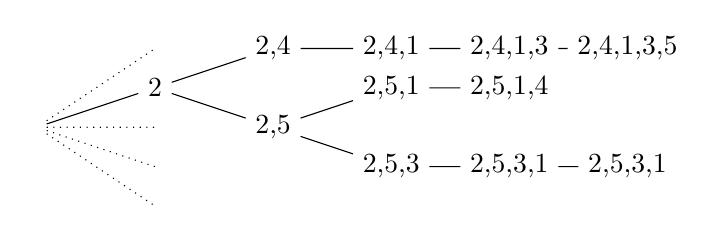
\begin{tikzpicture}[node distance=2cm]
\tikzstyle{level 1}=[sibling distance=0.5cm]
\tikzstyle{level 2}=[sibling distance=1cm]
	%    \tikzstyle{every node}=[draw]
    \node (root) {} [grow=right,dotted]
   	    child 
   	    child 
	    child 
    	child {node (2) {2} [black,solid]
	        child  {node (25) {2,5}
    	  		child {node (253)  {2,5,3}
    	  			child { node{2,5,3,1} child { node{2,5,3,1}} }
	      		}
    	   		child {node {2,5,1} child {node{2,5,1,4}}}        		        	          		        	  
	       	}
		    child {node {2,4}
		    	child {node {2,4,1}
		    		child {node {2,4,1,3} child {node {2,4,1,3,5} } }
		    	} 
		    }
	     }
	     child 
	 ;
%	\node at (253) {grid(1,1)};
\end{tikzpicture}
\caption{
Dette beslutningstræ viser backtracking efter at $2$ er valgt i række $1$. Blade i dybde $n$ angiver én løsning. Bemærk at roden er række 0.}
\label{fig:tree}
\end{figure}


\subsection{Bitmap-modellen}\label{bitmapmodellen}

\begin{figure}
\begin{center}
\begin{tabular}{|c|c|c|c|c|c}
\hline	0 & 0 & 0 & 1 & 0 \\
\hline	1 & 0 & 0 & 0 & 0 \\
\hline	0 & 0 & 1 & 0 & 0 \\
\hline	0 & 0 & 0 & 0 & 1 \\
\hline	0 & 1 & 0 & 0 & 0 \\
\hline
\end{tabular}
\end{center}
\caption{Samme eksempel som i \ref{fig:nq5eks}, men med en direkte binær repræsentation. En sat bit i en bitvektors position $i$ angiver en placering af en dronning i kolonne $i$.}
\label{fig:nq5eksbitmap}
\end{figure}

Idéen er beskrevet af \cite{Zongyan02} og implementeret af takaken \ref{nqueen.c}. Udover at repræsentere hver række på et skakbræt med en bitvektor, vedligeholdes der for hver række  en bitvektor \textbf{bitmap} for de pladser, hvor det er muligt at placere en dronning.  Tilladte pladser begrænses af tidligere placeringer, så der bruges 3 bitvektorer til holde styr på optagede pladser, \textbf{horisontal}, \textbf{venstrediagonal}  og \textbf{højrediagonal}.

Efter hvert valg, hvor den valgte placering sættes i en bitvektor \textbf{bit}, udregnes de nye bitvektore igen med følgende operationer.$\gg og \ll$ angiver et logisk skift, således at der altid indføres et $0$ fra henholdsvis højre og venstre.
\begin{description}
	\item[horisontal] $down \lor bit$ 
	\item[venstrediagonal] $(venstrediagonal \lor bit) \ll 1$
	\item[højrediagonal] $(højrediagonal \lor bit) \gg  1$\footnote{Java bruger $>>>$ for logisk højre skift. For venstre er logisk og aritmetisk ækvivalent}
	\item[bitmap]	$bitmap = \lnot(venstre \lor horisontal \lor højre)$	
\end{description}

Da træets højde er begrænset af $n$, er det maksimale pladsforbrug $antal\ bits\ per\ bitvektor \times antal\ af\ bitvektorer \times N$. For at håndtere N op til 32, kan vi nøjes med heltal der er repæsenteret af 32 bits til at repræsentere en bitvektor. Pladsforbruget for $N=26$ er så $32\times 26 \times 4 = 3328 bits$. Afhængig af implementationen og arkitekturens ordstørrelse vil dette variere. 

\subsection{Takakens algoritme}\label{takalgo}

For $Q(n)$ er mange løsninger spejlinger og roteringer af andre - og betragtes som en \textit{unik} løsning. Ved kun at betragte unikke løsninger, kan vi mindske antallet af blade i vores beslutningstræ \ref{fig:tree} til antallet af unikke løsninger, $S(n)$ og dermed mindske beregningstiden. I tabel \fixme{Tabel over Unikke løsninger vs. Totale antal løsninger} ses forskellen på antallet af unikke og totale løsninger. For hver løsning undersøges antallet af spejlinger og rotationer. Check funktion  \ref{nqueen.c} udfører dette.

Takaken opdeler beregningen i to delproblemer. Et hvor den første dronning placeres i øverste hjørne, og et andet delproblem hvor dronningen i den første række placeres i kolonnen $n/2$ til $2$. 

\begin{itemize}
	
\item Beskrivelse af hjørnebræt bound og dets implikationer
\item Beskrivelse af de andre delproblemer og dets implikationer
\item Husk at check ikke køres for hjørneproblemer = performance forskel
\end{itemize}

Disse optimeringer giver en hetorogen opdeling af delprobemer. Forholdet mellem antal løsninger og tid kan ses i \fixme{tabel/graf over antal løsinger og tid for hvert board}. Tidsforbrugt ved en profile kan ses \fixme{Java -Xprof kørses for n=1 til n=?, bliver Check= perrformance problem?}


\subsection{Parallelisering}\label{parrallel}

Et bræt med en eller flere valgte linjer kan løses på samme måde med takakens algoritme. Hvert delbræt kan løses uafhængigt og antallet af løsninger for hvert bræt akkumuleres for at få det totale antal løsninger.
Dette kan gentages for hver linje. Ved at oprette delbræt hvor M linjer allerede er valgt. Findes ca. (N-M)! delbræt skal der for N=26 vil der for M=3 være 26*25*24=15,600 delbræt.

Dette er en øvre grænse, der oprettes ikke delbræt som ikke er gyldige\fixme{not true}. Derudover er der i takakens kode optimeringer så der kun findes unikke løsninger (som så kan roteres og eller spejles) 


\section{\mig\ og \oc}\label{migogoneclick}
\begin{verse}
	Her beskrives \mig-grid og \oc\ overordnet. Tekniske detaljer i forbindelse med brug af \mig-grid, og særligt udvikling af \oc-applikationer, identificeres. Dette afsnit henvender sig således kun til dig, der ikke allerede har kendskab til disse emner.  
\end{verse}



\subsection{Minimum intrusion Grid}\label{mig}

\textsc{Minimum instrusion Grid}, herefter \mig, er et grid-system der sigter efter at stille så få krav for deltagelse som muligt - både overfor brugere og ressourcer. I \mig-termiologi er en ressource en enhed der kan sættes til at beregne et problem. I mange andre gridsystemer benyttes speciel software til kommunikation mellem den enkelte ressource og gridet, undgår man helt dette mindskes kompleksiteten af det samlede system dramatisk. Omkostninger til den første opsætning og efterfølgende vedligeholdelse af systemet minimeres. \fixme{beskrivelse af anonymitet, sikkerhed, skalerbarhed}. \mig er beskrevet indgåede i \cite{simplemig,mig}.

\mig\ giver brugeren mulighed for at få adgang til et stort antal beregningsressourcer, uden at skulle bekymre sig om hvor disse befinder sig, hvem der ejer dem, hvorvidt de hver især er istand til at løse den aktuelle opgave\footnote{Et givent problem kan f.eks. stille særlige krav til ressourcens arkitektur, eksisterende programmel, osv.}\fixme{er der mere under osv?}. Her og i det nedenstående henviser udtrykket ""brugeren"" til en udvikler der ønsker at få beregnet et problem vha. \mig \fixme{mindre fjollet definition}. Brugeren præsenteres for en abstraktion af \mig, der fremstiller et kendt paradigme fra unix-systemer; et hjemmekatalog hvori brugeren kan placere sine data- og programfiler. Brugerens interaktion med \mig\ forgår via en række scripts der efterligner kendte kommandoer til manipulation af filer i hjemmekataloget, og introducerer kommandoer til at starte og stoppe job. Begge metoder giver mulighed for at udføre basale funktioner på \mig, såsom at igangsætte job, se status på tidligere jobs og give adgang til data-, program- og resultatfiler i hjemmekataloget. Et job sættes igang ved at køre kommandoen migsubmit med såkaldt mRSL-fil\footnote{\mig\ Resource Language} der indeholder en beskrivelse af det job der skal afvikles. Beskrivelsen fortæller \mig\ hvilken programfil der skal køres, med hvilke parametre, hvor lang tid jobbet forventes at tage og eventuelle krav jobbet har til ressourcer der skal afvikle det. Et kørende job har adgang filerne i  hjemmekataloget. Resultatet af et job skal skrives til hjemmekataloget for senere at kunne aflæses af brugeren. For hvert job oprettes desuden 3 filer i hjemmekataloget. De indeholder hhv. exit-status, standard output og standard error, ganske som de kendes fra unix-systemer. 
Al den ovennævnte interaktion med \mig\ kan alternativt foregå gennem et særligt webinterface. 



\subsection{\oc}\label{applet}
\oc\ muliggører deltagelse i et \mig-grid uden andre forudsætninger end en webbrowser og java. Tilgengæld er denne metode begrænset til at afvikle programmer, der er tilgængelige som java-bytecode. Brug af \oc\ giver adgang til et enormt (potentielt) antal beregningsressourcer, hvilket er grunden til at benytte \oc\ i denne opgave.
\oc\ er et framework til udvikling af java-appletter, der kan interagere med \mig\. Ved hjælp af \oc\ kan en hvilken som helst computer gøres til en \mig-ressource, unden nogen for for opsætning eller installation af programmel, hvilket gør det muligt for ganske alm. mennesker at bidrage regnekraft til gridet. Det eneste der kræves er en webbrowser der kan afvikle java-appletter. Implementerer man sit job som en java-applet vil det kunne afvikles på alle \oc-ressourcer, uden at skulle specificere særlige krav til arkitektur med videre. Til gengæld vil det være begrænset til kun at køre på \oc-ressourcer. 
\oc\ er især interessant i forbindelse med hvad man kunne kalde sociale beregninger, det vil sige beregningsprojekter som almindelige mennesker kunne have interesse i at bidrage til, eller endog konkurrere om at bidrage mest til. Kendte eksempler på sådanne projekter er SETI@home og FOLDING@home. Når måling af tidsforbrug per ressource bliver implementeret i \oc\ kunne man også  forestille sig et \mig-grid som en åben markedsplads hvor både virksomheder og privatpersoner kunne købe og sælge regnekraft gennem \mig\ uden at skulle bekymre sig om, eller have mulighed for at vide, hvor beregningerne reelt foretages eller hvad hvad der regnes på. \fixme{for meget blah-blah}

\oc\ indeholder java-klasser til læsning og skrivning af filer i \mig\-hjemmekataloget samt checkpointing af det kørende job. 

Checkpoint foretages ved at serialisere det kørende job-objekt\footnote{\mig-applettens hoved objekt, der nedarver fra MiGJob-klassen} til en checkpoint-fil i hjemmekataloget på \mig. Det er altså kun objekt-variable der overlever på tværs af et checkpoint. I forhold til den rekursive backtrack-algoritme til \nq\ er det værd at bemærke at kald-stakken naturligvis ikke gemmes.

\subsubsection{\oc-specifikke begrænsninger}

I forbindelse med udvikling og afprøvning af en \oc-applet skal man være opmærksom på at Class-filer caches af browserens java-plugin. Ændringer i implementeringen kan medføre fejl under afviklingen på ressourcer der bruger forældede class-filer, selvom \mig opfatter jobbet som udført uden fejl. Ændringer i class-filer, der betyder opdatering af serialVersionUID, kræver opdatering af denne cache. Man kan altså riskikere at appletten får en undtagelse på serialVersionUID og derved markeres jobbet som færdigt, uden at være kommet til et resultat. En uhensigtsmæssighed i forbindelse med undtagelseshåndtering i basisklassen MigJob.java gør at jobbet alligevel vil se ud til at være afsluttet succesfuldt. Se afsnit \cite{bugs}. 

En java-applet afvikles i et lukket miljø, en såkaldt sandkasse, for at beskytte den maskine der afvikler appletten. n række begrænsinger vi bliver nødt til at forholde os til
\begin{itemize}
	\item Appletten kan maksimalt allokere 64MB hukommelse.
	\item Java's JNI (Java Native Interfaces) kan ikke benyttes fra appletter. 
	\item Ingen adgang til at læse/skrive lokale filer.
	\item Appletten er begrænset til kun at kunne oprette netværksforbindelser til den ip-adresse den er hentet fra.
	\item Ingen mulighed for at starte programmer på klient-maskinen.
	\item \oc\ Kode/Mininum intrusion.
\end{itemize}

Af disse er kun de to første af betydning for vores formål. Det bliver naturligvis et krav at alle delproblemer vi sender ud kan beregnes uden at bruge mere end 64MB hukommelse på klienten. Uden jni har vi ikke mulighed for måle på hvor meget reel cputid vores applet har fået tildelt, eller kende ressourcens hastighed eller arkitektur. 
\subsubsection{Checkpointing}
\oc\ indeholder kode til oprettelse af checkpoints under kørslen af et job. Et checkpoint er en gemt programtilstand, hvorfra det er muligt at fortsætte afviklingen. \oc\ indeholder desuden mekanismer til genetablering af programtilstanden fra et givent check. Når et \oc-job sendes til en ressource sendes det nyeste checkpoint med, hvis et sådant eksisterer, og \oc\ sørger for at genetablere tilstanden før eksekveringen af jobbet starter. Dette er præcis den funktionalitet vi behøver, for at kunne sikre at vi ikke behøver køre en beregning forfra når en ressource forsvinder.    




\section{Problemstørrelse og jobschedulering}
Et centralt emne ved parallelisering af algoritmer er partitionering af de data der beregnes på. Den ideelle opdeling definerer vi som en opdeling der sikrer at følgende gælder:
\begin{enumerate}
	\item Alle job har samme problemstørrelse - dvs. job tager samme tid at beregne.\label{beregningstid}
	\item Antallet af jobs er præcis lig antallet af ressourcer.\label{antal}
	\item Repræsentationen af job og resultater har minimal størrelse.\label{jobbeskrivelse}
\end{enumerate} 
Og med de yderligere antagelser at
\begin{enumerate}
	\item Ressourcer er homogene
	\item Ressourcer er permanente
\end{enumerate}
I denne ideelle situation opnåes maksimal udnyttelse af tilgængelige ressourcer, og samtidig minimalt overhead i forbindelse med jobskift og dataoverførsel.

I praksis er disse krav meget svære at opfylde. \ref{beregningstid} er for \nq\ ikke det samme som størrelsen af de del-data der regnes på. 
Som det ses på \ref{fig:todo} at beregningstiden for et delproblem stiger med antallet af løsninger i delproblemet. Vi kan altså ikke ikke ved opdeling af problemet kende de enkelte delproblemers beregningstid. Kunne vi det ville vi allerede kende antallet af løsninger. Istedet kan vi opdele problemet i dele med samme data-størrelse - dvs. samme antal dronninger mangler at blive placeret. 

\fixme{hvad kan vi sige om om beregningstiden for problemer med samme data-størrelse? Øvre grænse for variationen i køretid?} \fixme{indsæt reference til benchmarks, der viser beregningstid for hvert delproblem, og skriv noget om hvad benchmarks viser vi kan regne med ifm. beregningstid} 

Beregningstiden kompliceres yderligere af at delproblemerne skal beregnes på heterogene ressourcer, som vi ikke kan kende hastigheden af før delopgaven er færdigregnet. Heller ikke antallet af tilgængelige ressourcer (\ref{antal}) har vi ingen mulighed for at kende. Ydermere arver vi fra backtrack-algoritmen en opdeling af delproblemer i to typer, nemlig hjørnebræt og midtebræt. På grund af Takakens optimeringer har de to brættyper væsentligt forskellige beregningstider. 
\fixme{kun på grund af Takakens optimeringer?} 

I praksis gælder altså følgende:
\begin{itemize}
	\item Ressourcer er heterogene - både beregnings- og overførselstid. 
	\item Ressourcer er flygtige
	\item Antallet af ressourcer varierer
	\item Delproblemer er heterogene
	\
\end{itemize}



Vi kan sørge for at generere 

\fixme{beskriv vores løsning indgående}

\fixme{pointe : Antal job må (helst) aldrig blive mindre end antal ressourcer}

Idet både ressourcer og delproblemer er heterogene kan vi behandle dem som et samlet problem. Delopgaverne bliver så at sige bare endnu mere forskellige.
\fixme{pointe : den største forøgelse at samlet beregningstid vil forekomme hvis den langtsommeste ressource får den største delopgave når alle andre opgaver er regnet}

\fixme{Vi laver bræt med samme antal forudplacerede dronninger, og lader ønsket til antallet af bræt diktere antal forudplacerede dronninger - hvilke andre metoder kunne man benytte?}

Et N-dronning-job består af en .mRSL-fil og en  
\fixme{hvordan opretter vi job, hvad består et job af(serialize, mrsl)}

\fixme{Vi er nødt til at tage højde for at løsningen (antallet af løsinger) vil overstige hvad vi kan repræsentere som en 32bit værdi.}

Denne løsning kan bedst karakteriseres som såkaldt \emph{statisk orkestration}. Opdelingen i delproblemer er endeligt foretaget inden beregningen af delproblemer begynder. Som beskrevet er der et grundlæggende problem ved en statisk opdeling, nemlig at beregningen ikke kan tilpasse sig til en forøgelse af mængden af ressourcer. Istedet bliver man nødt til fra starten at generere nok opgaver til at kunne udnytte en eventuel ressourcetilgang. Samme problem opstår, på grund af heterogene ressourcer og opgaver, når antallet af delopgaver falder henimod slutningen af udregningen. 

For at afhjælpe dette problem kan joboprettelsen gøres mere dynamisk. Den indledende mængde delopgaver kan tilpasses det øjeblikkelige antal ressourcer. Herefter opdeles en eller flere af disse i mindre delopgaver, så snart der er ledige ressourcer. På denne måde sikres det at ingen beregningskraft står ubrugt hen. 
Det bedste valg af job til genopdeling vil være det jo der kræver mest beregningstid, da dette vil resultere i den mindst mulige spredning i beregningsstørrelse for de alle opgaver efter opdelingen. På figur \ref{tabel:boardtimes} ser vi eksempler for beregningstiden for hver delopgave. Det er tydeligt at de følger et mønster, og at vi kan bestemme et indbyrdes størrelsesforhold mellem hhv. alle hjørne- og midtebræt. Dette giver os en god idé om hvilken delopgave det bedst kan betale sig at splitte op. Tilgengæld har vi ikke mulighed for at vide, om beregningen af denne opgave allerede er ved at være færdig. 

Løsningen kører en separat tråd, der foretager checkpointing, og en timertråd, der giver giver beregningen besked om at afgive cpu'en til checkpointtråden, når den når et sikkert sted.

\section{Parallelisering af Takaken's nqueen I Java}

\subsection{Generelle implementeringsovervejelser}
\subsubsection{Opdeling af opgaver}


\subsubsection{Skemalægning af job}
I \mig skemalægges afviklingen af job som en FIFO-kø. Dvs. at job afvikles i samme rækkefølge som de submittes til gridet. Ved afbryding af jobbet eller ved udløb af tidsfristen for afvikling af jobbet placeres jobbet bagerst i køen.  




\subsubsection{Bugs og mangler}\label{bugs}
\begin{itemize}
	\item Et job fejler ikke hvis jobbet kaster en java.lang.Error (Forskellig fra Java.lang.Exception, begge har dog typen java.lang.Throwable)
	\item Ens job tvinges til at afhænge af MiG.nqueen.JoB
	\item File I/O følger ikke Inputstream / Outputstream	
	\item Brug af suns egen HTTP implementation. Brug i stedet http-commons fra Apache
	\item Vi har glemt en masse 
	\item Webstart vil klart være at foretrække. Det er rigtigt at der kommer en certifikat fejl (https) - men så længe certifikat ikke er i browserens CA liste vil browseren i stedet komme med en advarsel.q
\end{itemize}

I forbindelse med udvikling og afprøvning af en \oc-applet skal man være opmærksom på at Class-filer caches af browserens java-plugin. Ændringer i implementeringen kan medføre fejl under afviklingen på ressourcer der bruger forældede class-filer, selvom \mig opfatter jobbet som udført uden fejl. Ændringer i class-filer, der betyder opdatering af serialVersionUID, kræver opdatering af denne cache. Man kan altså riskikere at appletten får en undtagelse på serialVersionUID og derved markeres jobbet som færdigt, uden at være kommet til et resultat. En uhensigtsmæssighed i forbindelse med undtagelseshåndtering i basisklassen MigJob.java gør at jobbet alligevel vil se ud til at være afsluttet succesfuldt. Se afsnit \cite{bugs}. 


\subsection{Konkrete implementeringsproblemer}
\subsubsection{\mig\ job}\label{label}
\subsubsection{Iterative udgave}
\subsection{Checkpoint}

Fordi checkpointing gemmer ikke stack.

\subsection{Resultatindsamling og -visning}
En måde et holde styr på den samlede beregning af en løsning på \nq\ er, at have en vedligeholdelsesproces kørende, der sørger for at 
\begin{itemize}
	\item Genkøre fejlede job
	\item Indsamle resultater fra færdige jobs
	\item Muliggøre løbende projektstatus og offentliggørelse af resultater 
\end{itemize}
Dette program kan for eksempel være det samme der står for at oprette vores jobs i første omgang. Muligheden for at tilpasse ikke-kørte jobs på baggrund af informationer om gridets tilstand (antallet af tilgængelige ressourcer). 

Som alternativ tilbyder \mig-grid at informere indsendere når dennes job er afsluttet, eksempelvis via email. Det vil være betydeligt enklere kun at foretage behandling af resultater hver gang et sådant er klar, uden at have et permanent indsamlingsprogram kører. Vi er dog stadig nødsaget til at håndtere fejl i det enkelte job eller rapporteringen af jobafslutning. 

- Frej Lad \mig sende en mail pr. færdigt job? Og så et job der checker 'jævnligt' at alle mails er modtaget?



\section{Implementeringens struktur}\label{implementeringensstruktur}
\begin{verse}
	Følgende er ment som en læsevejledning til programmets kildekode, såvel som en vejledning til afvikling af programmet med forskellige formål. 
\end{verse}

Den udviklede kildekode er organiseret i følgende filer:
\begin{description}
	\item[Board.java] 
	\item[Board2.java] Basis-klasse for wrapper-klasser til backtrack
	\item[CornerBoard.java] wrapper-klasse til backtrack for cornerboards
	\item[MiddleBoard.java] wrapper-klasse til backtrack for middleboard
	\item[CheckPointer.java] implementerer checkpointing
	\item[CheckPointAction.java] implementerer checkpointing
	\item[CornerBoardBoardTest.java] unittests til CornerBoard
	\item[MiddelBoardTest.java] unittests til MiddleBoard
	\item[MiGClient.java] java-implementation af en del af \mig-grid-hjælpeprogrammerne
	\item[MiGJob.java] klasse der beskriver et job og kan generere en .mRSL-fil
	\item[MiGSSLSocketFactory.java] hjælpeklasse til MiGClient-klassen
	\item[NQueenBoards.java] Jobgeneratoren, parallel-nqueen-algoritme, der genererer delproblemer i form af boards, hvor de første $m$ dronninger allerede er placeret. 
	\item[NQueenJob.java] hovedklassen for et \mig-grid-\oc-job. 
	\item[NQueens.java] Testfil - Direkte java-port af Takakens c-kode. Kan køres som \oc\ job.
	\item[NQueensL.java] Testfil - Direkte java-port af Takakens c-kode. Kan køres lokalt.
\end{description}

Programmet kan afvikles lokalt på en enkelt maskine eller på \mig-grid,  



\section{Afprøvning og benchmarking}
%Benchmarking-delens fremmeste formål er at finde svar på en række spørgsmål inden udregningen sættes igang.
%Reelt har vi kun en enkelt parameter vi kan skrue på, nemlig $m$ - antallet af dronninger vi placerer på hver board før vi genererer et \mig\ job til at regne videre på det board. 
%Hvilket forhold mellem 

%\subsection{Takaken}
%\subsection{Java port}
%\subsection{Java port v2}
%\subsubsection{Rekursion vs. Iterativ metode}
%\subsubsection{Iterativ med checkpoints}
%\subsection{MiGrid}

Benchmarking-delens fremmeste formål er at finde svar på en række spørgsmål
inden udregningen sættes igang.  Reelt har vi kun en enkelt parameter vi kan
skrue på, nemlig $m$ - antallet af dronninger vi placerer på hver board før vi
genererer et mig job til at regne videre på det board.  Hvilket forhold mellem 
\fixme{what?}
%\subsection{Takaken}
%\subsection{Java port}
%\subsection{Java port v2}
%\subsubsection{Rekursion vs. Iterativ metode}
%\subsubsection{Iterativ med checkpoints}
%\subsection{MiGrid}

\subsection{Lokale tests}

Vi starter med at teste de forskellige udgaver af koden lokalt, så vi har en
baseline at sammenligne med.

Alle lokale tests er kørt på en IBM T43, med en pentium m 1.86Ghz cpu, 

Java koden er kompilet med javac

\begin{verbatim}
alex@roadrunner:~/temp/queens/src/main/java$ javac -version
javac 1.5.0_11
\end{verbatim}

C koden er kompilet med \texttt{gcc -Os -O2 -o nq nqueens.c}

\begin{verbatim}
alex@roadrunner:~/temp/queens/src/main/java$ gcc --version
gcc (GCC) 4.1.2 (Ubuntu 4.1.2-0ubuntu4)
\end{verbatim}

De første tests er kørt på revision 77 (i forbindelse med den iterative test er
udskrivning af debug info til skærmen dog blevet kommenteret ud)

\begin{figure}[h]
\begin{center}
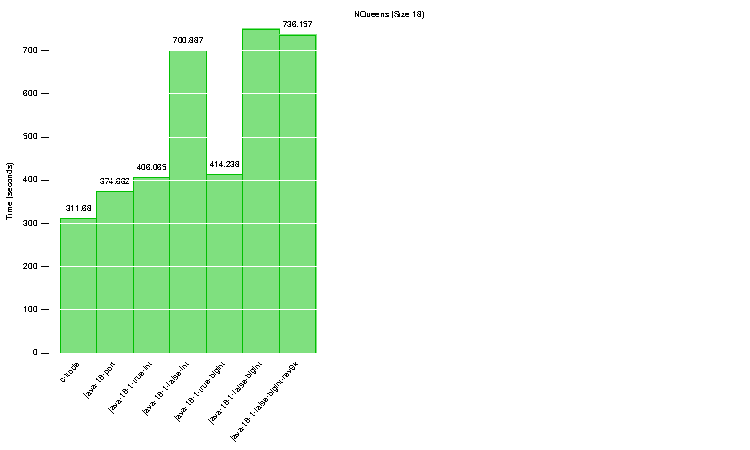
\includegraphics{../benchmarks/lokal.pdf}
\caption{insert proper caption here } 
\label{figur:lokal}
\end{center}
\end{figure}
\fixme{caption, or no caption.. this graph is redundant information}

Som det ses er C udgaven en smule hurtigere end den direkte java port, der igen
er lidt hurtigere end den paralleliserede udgave af koden, når den kører
rekursivt. Den iterative udgave er væsentlig langsommere..

Den parallelle udgave af koden er i dette tilfælde her kørt med
\texttt{maxSteps} på 1. 
\begin{figure}[h]
\begin{center}
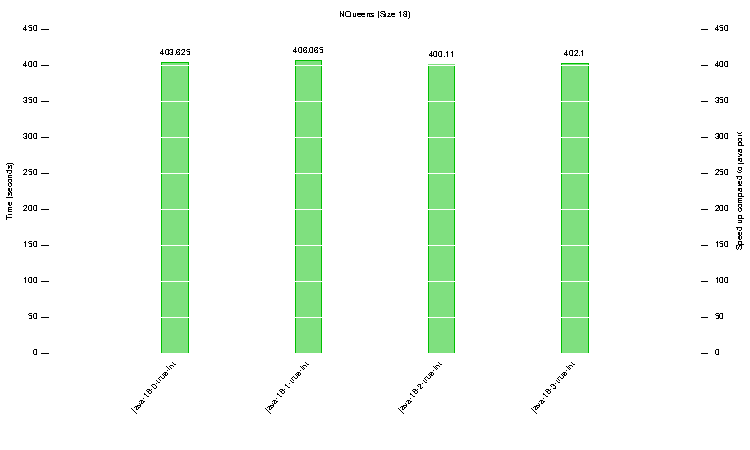
\includegraphics{../benchmarks/maxsteps.pdf}
\caption{insert proper caption here } 
\label{figur:maxsteps}
\end{center}
\end{figure}

På figur \ref{figur:maxsteps} er vidst kørsler for $n=18$ for forskellige
$maxSteps$. 
Som det ses, har det ikke den store indflydelse på performance hvor stor
$maxSteps$ er, der er altså ikke det store overhead ved at generere en masse
opgaver og løse dem bagefter, når det kører lokalt. 

Det skal også nævnes at for $maxSteps>n/2$ vil vores program regne forkert.
Dette skyldes \fixme{ja.. hvad skyldes det.. }


I tabel \ref{tabel:noboards} kan det ses hvor mange boards der bliver genereret
for forskellige $n$ og $maxSteps$. 

\fixme{hvor mange jobs bliver der lavet for de forskellige maxsteps, indsæt
tabel?}
\begin{table}
	\begin{center}
		\begin{tabular}{|c|c|c|c|c|c|}
			\hline N  & maxSteps  & boards & n  & maxSteps & boards \\
			\hline 15 & 0         & 18     & 17 & 0        & 21     \\
			\hline 15 & 1         & 173    & 17 & 1        & 243    \\
			\hline 15 & 2         & 1310   & 17 & 2        & 2282   \\ 
			\hline 15 & 3         & 8349   & 17 & 3        & 18161  \\
			\hline 15 & 4         & 43961  & 18 & 0        & 23     \\
			\hline 16 & 0         & 20     & 18 & 1        & 289    \\
			\hline 16 & 1         & 212    & 18 & 2        & 2983   \\
			\hline 16 & 2         & 1797   & 18 & 3        & 26204  \\
			\hline 16 & 3         & 12840  &    &          &        \\
			\hline 16 & 4         & 76224  &    &          &        \\
			\hline
		\end{tabular}
		\caption{Antal Boards der bliver genereret}
		\label{tabel:noboards}
	\end{center}
\end{table}

Alle tests er i første omgang kørt 5 gange, dette blev gjort for at se om
køretiden svingede meget, da dette ikke lader til at være tilfældet (se figur
\ref{figur:b1} vil resten af testene kun blive kørt 1 gang.. 

\begin{figure}[h]
\begin{center}
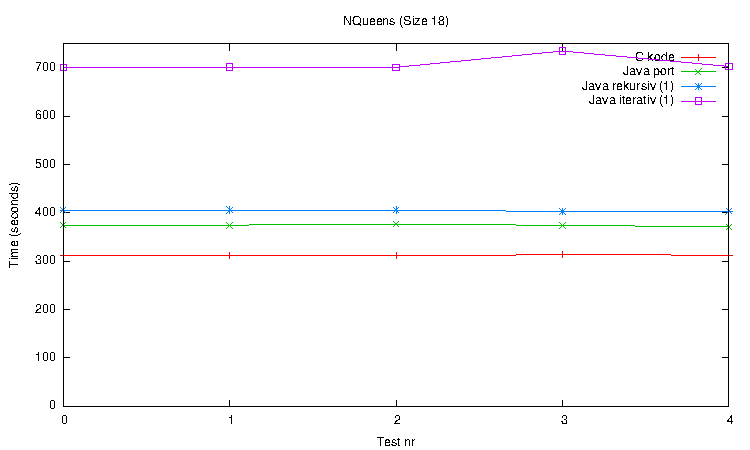
\includegraphics{../benchmarks/b1.pdf}
\caption{insert proper caption here } 
\label{figur:b1}
\end{center}
\end{figure}

Nu skal vi så se på hvor hurtigt det kører når vi smider det efter MiGrid. 
Disse tests er kørt med \texttt{maxSteps} 0 og 1.

\fixme{indsaet en graf, eller bare resultaterne og henvis til b3?}
De foregående tests er kørt med kode der bruger \texttt{int} til at gemme resultaterne,
i de næste tests er \texttt{int} skiftet ud med \texttt{BigInteger} (revision
83
\clearpage
Sammenligning af alle benchmarks

Som det ses på figur \ref{figur:lokal} kører den iterative udgave af koden fra
rev. 83 (med bigint) utroligt langsomt i forhold til foregående udgaver.  Dette
skyldes en en linje kode, der ikke var blevet kommenteret ud. Denne linje
konkatenerede to strenge. Uden denne linje kører koden væsentlig hurtigere, som
det kan ses på den sidste søjle i figur \ref{figur:lokal}


Som det kan ses på figur \ref{figur:lokal} kører den rekursive kode en smule
langsommere med \texttt{BigInteger} end med \texttt{int}, hvor tiden stiger fra
406.xxx til 414.xxx\fixme{indsaet rigtige tal}, hvilket svarer til en forøgelse
på knap 2\%

\subsection{overhead ved jobskifte}

I MiG\_main() metoden i NQueenJob laver vi et timestamp i starten og slutningen
af metoden.  og kan så tage start tiden for et job og trække sluttiden for det
foregående job fra, og man har så et estimat for hvor lang tid et jobskifte
tager, vi har gjort dette for 8 jobs, og får så 7 estimater, gennemsnittet af
dem bliver 18.455 sek.  Op til 15 af disse 18 sekunder, skyldes at oneclick
applet'en sover i 15 sekunder.  Ved en kørsel med $n=18$ og $maxSteps=1$, hvor
vi så får 289 jobs, giver det knap 89 minutter. 

\subsection{kald til backtrack}

Hvis man ser på antallet af kald til backtrack de forskellige versioner laver,
er de ens for c koden og den direkte java port, og hvis man kører med
$maxSteps=0$ er antallet af kald for den parallele og iterative kode også det
samme som for c koden (se tabel \ref{tabel:backtrackkald}. Med $maxSteps>0$ får
vi færre kald til backtrack, hvilket skyldes at en del af disse kald bliver
lavet i forbindelse med oprettelsen af de ekstra boards. 

\begin{table}
\begin{center}
\begin{tabular}{|c|c|c|c|}
\hline 18 & C kode        &             &             \\
\hline 18 & Java          &             &             \\
\hline 18 & Java rek. &             &             \\
\hline 18 & Java ite. &             &             \\
\hline
\end{tabular}
\caption{Kald til backtrack}
\label{table:backtrackkald}
\end{center}
\end{table}
\fixme{indsæt tal (*07-01*)}

\subsection{Jobstørrelse}

Med jobstørrelse refererer vi til hvor lang tid det tager at løse et job, og
ikke størrelsen på data. 
Som det ses i \ref{tabel:jobsize}, varierer jobstørrelsen
meget. Cornerboards er generelt ret små, mens middleboards er generelt er en del
større. Det ses også i tabellen at jobstørrelsen afhænger af de bounds der er i
henholdsvist MiddleBoard og CornerBoard. Hvis man øger $maxSteps$ og dermed får
lavet flere jobs, ses det at de enkelte jobs bliver delt op i nogenlunde lige
støre dele, den relative størrelse mellem det mindste og største jobs er dog
stadig nogenlunde det samme. \fixme{lav en benchmark/beregning der viser dette?}

\subsection{Generering af jobs}

Generering og indsendelse af jobs afhænger tildels af den internetforbindelse
man sidder på, da indsendelse jo går via internettet. De forskellige jobs vi har
submitted til MiGrid har genereringen og indsendelse af jobs svinget fra xx til
xx (se tabel \ref{tabel:jobgenerering}) \fixme{lav den fscking tabel og skriv de
rigtige tal ind}. Langt den største del af tiden går også med at sende jobsne,
da genereringen af jobs for større mængder jobs tager ca 0.01ms/job
\begin{verbatim}
18: 4, 6, 44, 280
18: 23, 289, 2983, 26204
18: 0.17, 0.02, 0.01, 0.01
17: 4, 6, 23, 206, 1252
17: 21, 243, 2282, 18161, 121116
17: 0.19, 0.02, 0.01, 0.01, 0.01
\end{verbatim}
\fixme{lav det om til en tabel.. der}

TODO MiGrid
\section{Forbedringer til \oc\ og \mig}
%\input{forbedringer.tex}
\fixme{TODO}
langsom til at sende resultatet til serveren hvis browseren dør mens den er ved
at sende resultatet til serveren, er det ikke sikkert den når at smide hele

\oc applet'en cacher class filer, s hvis man har ænret i sin kode og
uploadet nye class filer bliver man nødt til at lukke browseren helt ned og
starte den op igen, hvis man vil have den til at loade de nye class filer, lader
det umiddelbart til.. 

\oc applet'en kommer hele tiden med en popup fejl, hvis brugeren ikke har
certificat (skal nok lige verificeres, var noget jeg fik at vide af Asser, da
han legede ressource for \mig)

Job Status side ala. Files/Folders
tingen, så man nemmere kan vælge flere jobs og cancelle/resubmitte.. og
wildcards til migcancel.py ville også være en go ting, så man kunne lave en
migcancel.py *14\_37* fx.. 

vis queued/cancelled/finished/executing/m.fl jobs ville også være en brugbar feature

mulighed for at slette job helt, så ens jobstatus side ikke er så stor.. eller
"pensionere" dem

Den dræber nogen gange jobs, dette ser ud til at ske, hvis den lige har
færdiggjort job <jobid>, og så (af en eller anden årsag) prøver at hente det
\_samme\_ job igen, så bliver dette job (sjovt nok) slået ihjel af serveren, og
så sleeper applet'en i 80s før den prøver igen.. 

Errors bliver ikke fanget
\begin{verbatim}
checkpoint_request_url_str: https://mig-1.imada.sdu.dk/sid_redirect/7bc01a0e4ead439c63c84fd149eb93ac325fdf1809aedc23049c010890bf14bd/13768_6_2_2007__8_42_57_mig-1.imada.sdu.dk.0.NQueenJob.checkpoint.latest
Exception in thread "Thread-18" java.lang.NoClassDefFoundError: CheckPointAction
	at java.lang.Class.getDeclaredMethods0(Native Method)
	at java.lang.Class.privateGetDeclaredMethods(Class.java:2427)
	at java.lang.Class.getMethod0(Class.java:2670)
	at java.lang.Class.getMethod(Class.java:1603)
	at MiG.oneclick.Exe.getJobMethods(Exe.java:73)
	at MiG.oneclick.Exe.run(Exe.java:236)
	at java.lang.Thread.run(Thread.java:619)
sendJobFinished
\end{verbatim}

%\bibliographystyle{plainnat}

lo
\bibliography{rapport,nqueens}

\appendix
%\landscape
%\tiny


\section{Kildekode}
\subsection{nqueens.c}\label{nqueen.c}
%\verbatiminput{../../nqueens.c}

\section{Synopsis}
%\documentclass[a4wide,10pt]{article}

\usepackage[danish]{babel}
\usepackage[latin1]{inputenc}
\usepackage{verbatim}
\usepackage{amsmath}
\usepackage{lscape}
\usepackage{multicol}

\title{Bachelorprojekt\\Synopsis\\N-dronning problemet i MiG}
\author{Thomas Clement Mogensen \\ Frej Soya \\ Alex Esmann }

%\maketitle
\begin{document}
\maketitle

\subsection*{Problemformulering}
Opgavens formål er at implementere en parallel udgave af Takakens algoritme til løsning af n-dronning-problemet. Algoritmen skal køre på MiG-systemet (Minimum Intrusion Grid) og MiG's one-click arkitektur skal kunne udnyttes til at skaffe ressourcer til beregning af problemet. Formålet er på langt sigt at få beregnet en løsning til N-dronning-problemet for $n=26$, men opgaven er kun at gøre dette muligt ved hjælp af MiG. N-dronning-problemet er et klassisk beregningsproblem, der går ud på at finde antallet af mulige måder n dronninger kan placeres på et "skakbræt" med n x n felter, uden at nogen af dem er istand til at slå hinanden i næste træk. Problemets størrelse stiger eksponentielt med n, og er uhyre beregningstungt for store n, hvorfor store distribuerede systemer ofte benyttes. Hidtil er der kun fundet løsninger for $n \in \{1,...,25\}$. For distlab-gruppen her på diku ville en løsning for $n=26$, beregnet på et MiG-grid, kunne skabe opmærksomhed omkring MiG-systemet. 

MiG er beskrevet indgående i \cite{simplemig} og \cite{mig}, \cite{etsi} beskriver N-dronning-problemet grundigere end ovenstående og præsenterer en løsning for n=25. Appendix queens.c i \cite{etsi} er en udskrift af Takakens algoritme implementeret i C.
One-click muliggør deltagelse i et MiG-grid uden andre forudsætninger end en webbrowser og java. Tilgengæld er denne metode begrænset til at afvikle programmer, der er tilgængelige som java-bytecode. Brug af one-click giver adgang til et enormt (potentielt) antal beregningsressourcer, hvilket er grunden til at benytte one-click i denne opgave.    

Opgaven indeholder altså følgende delproblemer: 
\begin{itemize}
\item At finde en effektiv strategi til parallelisering af Takakens algoritme. Herunder overvejelser omkring den optimale størrelse på delproblemer.
\item Implementation af algoritmen i java på en sådan måde at den kan afvikles af one-click-klienter. 
\item Strategi for indsamling, behandling og præsentation af delresultater. 
\item Første opgave er naturligvis at få et bedre kendskab til MiG.
\end{itemize}

Projektets form�l er ikke at beregne en l�sning til N-dronning-problemet for $n=26$, hvilket problemets beregningsm�ssige omfang kombineret med tids- og ressourcebegr�sninger udelukker i praksis. Men kun at muligg�re og forh�bentlig igangs�tte denne beregning. 
Vi vil ikke tage stilling til den benyttede algoritmes korrekthed eller effektivitet, men kun til den bedst mulige strategi for parallelisering. Partitionering af problemdata skal foreg� p� en fornuftig m�de, med tanke p� hvordan det forventes beregningsressourcerne opf�rer sig, men en decideret statisk unders�gelse af midlertidige MiG-ressourcers opf�rsel eller levetid vil ikke blive foretaget\footnote{Med ressourcers opf�rsel t�nkes p� den tid man kan forvente en bruger vil lade sin one-click-klient k�re}. Fordele og ulemper ved MiG eller One-click i forhold til andre grid-systemer falder ogs� udenfor opgavens omfang. 


\begin{thebibliography}{99}
\bibitem{simplemig} Karlsen, Henrik Hoey, Vinter, Brian:
\emph{Minimum intrusion Grid - The simple model},
http://mig-1.imada.sdu.dk/MiG/Mig/published\_papers/ETN05-Simple.pdf (2005)
\bibitem{mig} Vinter, Brian:
\emph{The Architecture of the Minimum intrusion Grid, MiG},
http://mig-1.imada.sdu.dk/MiG/Mig/published\_papers/CPA05-Arch.pdf
(2005)
\bibitem{etsi} Guillemin, Patrick:
\emph{3rd N Queens ETSI Plugtests Contest - Counting the number of
  solutions Single and Distributed Programs}
http://portal.etsi.org/docbox/GRID/Open/GRID\%20Plugtests\%202006/N-QUEENS-TESTCASE-2006-v2.pdf (2006)
\end{thebibliography}

%\landscape
%\tiny
%\begin{multicols}{2}[\section{\LaTeX kildekode}]
%\section*{Skabelon.tex}
%\verbatiminput{skabelon.tex}
%\end{multicols}

\end{document}



%\landscape
\begin{multicols}{2}
\tiny
\section{Benchmark Output}
zomg.. benchoutput should be here.. 
\end{multicols}

%\begin{multicols}{2}[\section{\LaTeX kildekode}]
%\section*{Skabelon.tex}
%\verbatiminput{skabelon.tex}
%\end{multicols}


\end{document}
